\documentclass[10pt,twocolumn,a4paper]{article}

\usepackage[utf8]{inputenc}
\usepackage[T1]{fontenc}
\usepackage{times}
\usepackage{graphicx}
\usepackage{amsmath}
\usepackage{amssymb}
\usepackage{geometry}
\usepackage{url}
\usepackage{booktabs}

\geometry{
	a4paper,
	left=1.6cm,
	right=1.6cm,
	top=1.8cm,
	bottom=2.0cm,
	columnsep=0.7cm
}

\setlength{\parindent}{0.35cm}
\setlength{\parskip}{0pt}

\title{\textbf{Tiny CNN vs.\ YOLO for Chess Piece Recognition:\\ An Efficiency-Oriented Comparison on Synthetic Boards}}

\author{
	Honi Arora\\
	Bachelor's Degree Programme in Applied Computer Science and Artificial Intelligence (ACSAI)\\
	Course: AI-LAB -- Computer Vision, Signal Processing, and Natural Language Processing\\
	Department of Computer Science, Sapienza University of Rome\\
	Matricola: XXXXXXX\\
	\texttt{arora.XXXXXXX@studenti.uniroma1.it}
}

\date{}

\begin{document}

	\maketitle

	\begin{abstract}
		We study a simple but practical question: to read the pieces on a chess board image, do we really need a full object detector, or is a small image classifier enough? We compare two paradigms on the same synthetic data: a compact, from-scratch convolutional neural network (CNN) that classifies individual board cells, and YOLOv8 object detectors of three sizes that find and classify pieces directly. The shared source is the \textit{Chess Positions} dataset, whose rendered boards have a perfect $8\times8$ grid; we derive $50\times50$ cell crops for the CNN and grid-aligned bounding boxes for YOLO from the same labels, and we evaluate both with a common ``occupied-cell accuracy''. Our CNN is tuned with Optuna and tracked with Weights \& Biases. The main finding is that a $28{,}813$-parameter CNN reaches $99.96\%$ per-piece accuracy, statistically tied with a pretrained YOLOv8n at $100\%$, while being about $93\times$ smaller, $8.5\times$ faster, and $45\times$ lighter on disk; a sub-nano YOLO trained from scratch collapses to $20.7\%$. The contribution of the project is a controlled, reproducible benchmark with a fair cross-paradigm metric, a hyperparameter study that explains \emph{why} the tiny model wins, and a discussion of when each paradigm is the right tool.
	\end{abstract}

	\noindent\textbf{Keywords:} artificial intelligence; deep learning; computer vision; image classification; object detection; hyperparameter optimization.

	\section{Introduction}

	Recognizing the pieces on a chess board from an image is a useful sub-task for digitizing games, building tutoring tools, or streaming over-the-board play. There are two natural ways to attack it. The first is \emph{image classification}: if we already know where each square is, we can cut the board into 64 cells and ask a model ``what piece is in this cell?''. The second is \emph{object detection}: feed the whole image to a model that must simultaneously \emph{locate} each piece with a bounding box and \emph{label} it. Modern detectors such as YOLO~\cite{redmon2016yolo,jocher2023yolov8} are the standard choice for the second formulation, while convolutional networks~\cite{lecun2015deep,krizhevsky2012alexnet,he2016resnet} are the standard choice for the first.

	The two paradigms have very different costs. A detector is powerful and works on messy, unconstrained photos, but it is also heavier and slower. A classifier is cheap, but it assumes the object is already isolated. In many practical projects people reach for a detector by default, even when the input is highly structured and the localization is essentially free. This is the gap we examine.

	In this project we do not propose a brand-new architecture. Our contribution is a \emph{careful, controlled comparison}: we train a small custom CNN and three YOLOv8 variants on \emph{the same} data, measure them with a \emph{single fair metric}, and analyze the accuracy/compute trade-off. Concretely, we (i) design a data pipeline that turns one labelled dataset into two consistent views; (ii) run a hyperparameter search on the CNN and report what actually matters; (iii) include a deliberately under-sized ``pico'' detector to test whether simply shrinking a detector is a good idea; and (iv) report deployment-oriented numbers (parameters, FLOPs, latency, disk size), not only accuracy.

	The rest of the report is organized as follows. Section~\ref{sec:related} reviews the relevant background. Section~\ref{sec:method} describes the pipeline and the models. Section~\ref{sec:setup} gives the experimental protocol and presents and discusses the results. Section~\ref{sec:conclusion} concludes.

	\section{Related Work}
	\label{sec:related}

	\textbf{Classical board recognition.} Early chess-vision systems relied on hand-crafted steps: detecting the board with line/corner detection, warping it to a frontal view, and classifying squares with template matching or simple features. These pipelines are fast but brittle to lighting, piece sets, and viewpoint.

	\textbf{Convolutional classification.} Deep CNNs replaced hand-crafted features for image classification~\cite{lecun2015deep}. AlexNet~\cite{krizhevsky2012alexnet} and residual networks~\cite{he2016resnet} are the canonical examples. For a task as visually clean as rendered chess pieces, a small CNN with convolutional, batch-normalization~\cite{ioffe2015batchnorm}, and dropout~\cite{srivastava2014dropout} layers is more than sufficient, which motivates our compact design.

	\textbf{Object detection.} Single-stage detectors like YOLO~\cite{redmon2016yolo} predict boxes and classes in one forward pass; the Ultralytics YOLOv8 family~\cite{jocher2023yolov8} provides easy-to-train models pretrained on COCO~\cite{lin2014coco}. Detection is the right tool when pieces must be \emph{found}, not just named.

	\textbf{Datasets.} We use the \textit{Chess Positions} dataset~\cite{koryakin2019chess}, a large set of rendered boards labelled by the FEN string in each filename. Because the board fills the frame, the geometry is known exactly, which makes it an ideal controlled setting to compare classification against detection without the confound of board localization.

	\textbf{Hyperparameter optimization.} Rather than tuning by hand or with grid search, we use Optuna~\cite{akiba2019optuna}, a framework that samples configurations and prunes weak trials; random/efficient search is known to beat grid search at equal budget~\cite{bergstra2012random}.

	\textbf{How we differ.} Prior work typically commits to one paradigm. We instead hold the data and the evaluation fixed and compare both, adding an explicit efficiency axis and a hyperparameter analysis that explains the outcome.

	\section{Methodology}
	\label{sec:method}

	The complete pipeline is shown in Fig.~\ref{fig:architecture}. A single labelled dataset is turned into two consistent ``views'' so that the classifier and the detector are trained and evaluated on exactly the same underlying information.

\begin{figure*}[t]
	\centering
	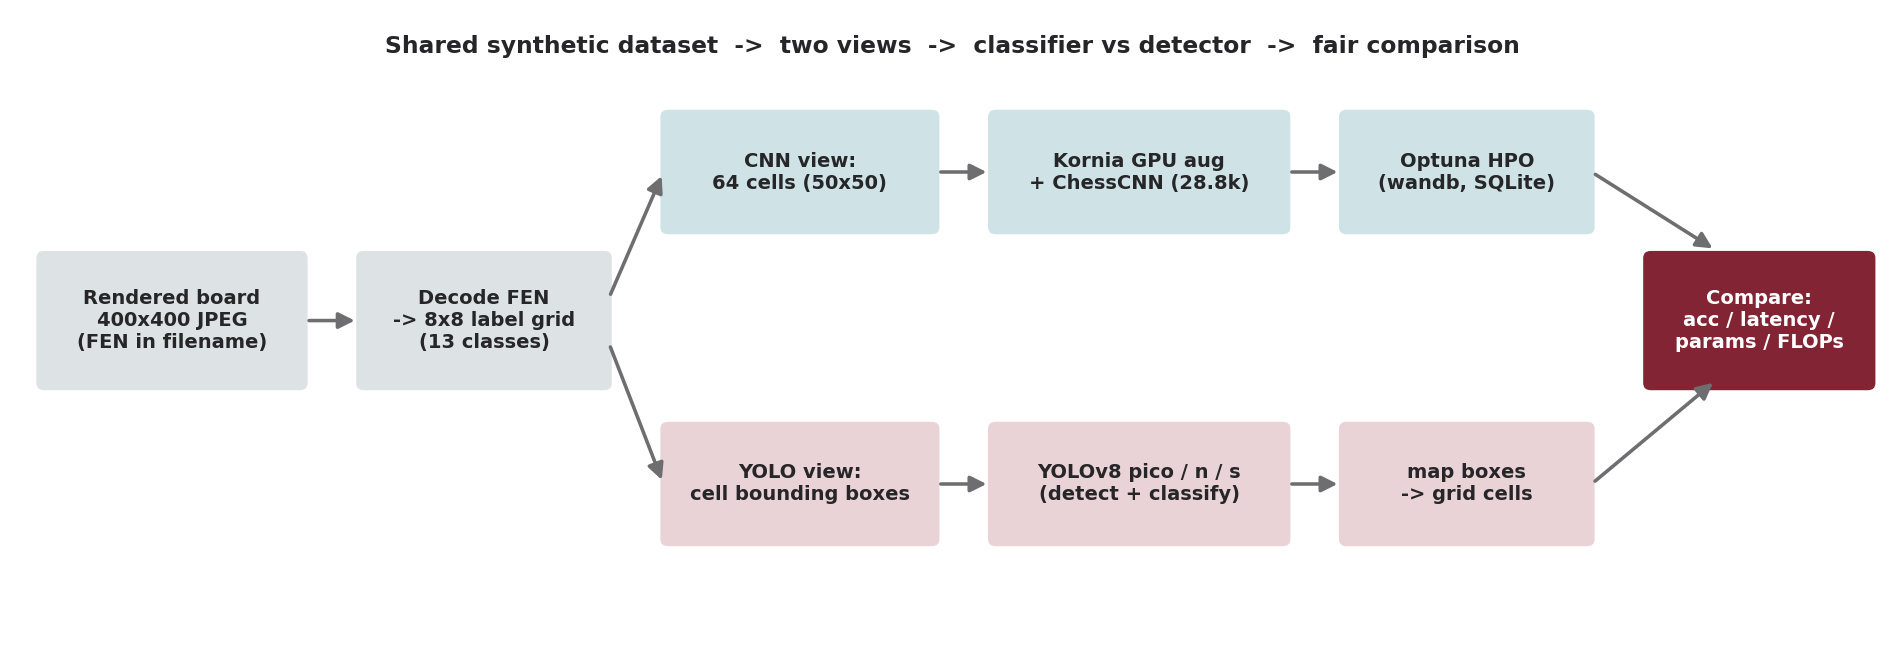
\includegraphics[width=0.95\textwidth]{01-Architecture.png}
	\caption{Pipeline. A rendered board is decoded from its FEN filename into an $8\times8$ label grid. From this single grid we build two views: $50\times50$ cell crops for the custom CNN (trained with Kornia GPU augmentation and tuned with Optuna), and grid-aligned bounding boxes for the YOLOv8 detectors. Both branches are evaluated with the same occupied-cell accuracy and with deployment metrics (parameters, FLOPs, latency, disk size).}
	\label{fig:architecture}
\end{figure*}

	\subsection{Data and preprocessing}

	Each image is a $400\times400$ rendered board, and its label is the FEN (Forsyth--Edwards Notation) string in the filename, with the rank separator \texttt{/} replaced by \texttt{-}. We parse the FEN into an $8\times8$ grid of class indices (empty $=0$; white pieces $1$--$6$; black pieces $7$--$12$). Because the board fills the frame, each cell is exactly $50\times50$ pixels. From the grid we derive:
	\begin{itemize}
		\item \textbf{CNN view:} 64 cell crops per board, each with its class (13 classes including ``empty'').
		\item \textbf{YOLO view:} one bounding box per \emph{occupied} cell, equal to that cell rectangle, with 12 piece classes (detectors do not predict ``empty'').
	\end{itemize}
	The boards are strongly imbalanced ($\approx 83\%$ of cells are empty), so for the CNN we cap the number of empty cells to roughly the number of piece cells per board, giving about $429{,}000$ balanced crops, and we report accuracy on occupied cells only. To keep training fast we precompute the crops once into a memory-mapped array, so each training step reads a $50\times50$ patch without re-decoding the JPEG. On-the-fly augmentation (small affine, colour jitter, noise, blur) is applied on the GPU with Kornia~\cite{riba2020kornia}, with the augmentation strength treated as a tunable hyperparameter.

	\subsection{Models}

	\textbf{Custom CNN.} A small from-scratch network: three convolutional blocks (Conv$\to$BatchNorm$\to$ReLU$\to$MaxPool) with $16$, $32$, $64$ channels, followed by global average pooling and a two-layer classifier with dropout. The final model has only $28{,}813$ parameters. The architecture size (number of blocks, channel width, hidden size, dropout) is part of the hyperparameter search rather than fixed by hand.

	\textbf{YOLO detectors.} We use three YOLOv8 variants~\cite{jocher2023yolov8}: \texttt{yolov8n} and \texttt{yolov8s} initialised from COCO-pretrained weights~\cite{lin2014coco} (transfer learning), and a custom width-scaled ``pico'' model ($\approx$ one quarter the width of nano) trained \emph{from scratch}, since no pretrained sub-nano weights exist. The pico model is included on purpose, to test whether shrinking a detector to classifier size is a sensible strategy.

	\textbf{What is reused vs.\ ours.} The YOLOv8 implementation and its pretrained weights are reused from Ultralytics; PyTorch~\cite{paszke2019pytorch}, Optuna~\cite{akiba2019optuna}, and Kornia~\cite{riba2020kornia} are standard libraries. Everything else---the data pipeline and two-view derivation, the custom CNN, the augmentation strategy, the hyperparameter study, the pico scaling, and the unified evaluation---is our own work.

	\subsection{Objective and training strategy}

	The CNN is trained with the cross-entropy loss. The architecture and optimization hyperparameters are searched with Optuna using a persistent (resumable) study and median pruning; every trial is logged to Weights \& Biases. The search covers the learning rate and weight decay (log scale), the optimizer (Adam~\cite{kingma2015adam}, AdamW~\cite{loshchilov2019adamw}, SGD), the augmentation strength, and the network shape. A short calibration run measures the per-step time and predicts the total training time before each run. The best configuration is then retrained and saved. The YOLO models are trained with the Ultralytics default recipe (its automatic optimizer selects AdamW), the same image size for all variants, and a fixed data fraction so that training time stays comparable.

	\section{Experimental Setup}
	\label{sec:setup}

	\subsection{Dataset}

	We use the \textit{Chess Positions} dataset~\cite{koryakin2019chess}. To bound compute we work with a subset of $20{,}000$ training and $4{,}000$ test boards; the test boards are never seen during training or tuning. Table~\ref{tab:dataset} summarizes the data. The main limitation is that the images are \emph{rendered}, not photographed: pieces are clean and perfectly aligned, which is favourable to a cell classifier and removes the board-localization problem that a real photo would introduce.

	\begin{table}[h]
		\centering
		\caption{Dataset summary.}
		\label{tab:dataset}
		\begin{tabular}{|l|c|}
			\hline
			\textbf{Property} & \textbf{Value} \\
			\hline
			Dataset name & Chess Positions~\cite{koryakin2019chess} \\
			Source / license & Kaggle / CC0 \\
			Training boards & 20{,}000 \\
			Test boards & 4{,}000 \\
			CNN classes & 13 (empty + 12) \\
			YOLO classes & 12 (pieces) \\
			Input format & $400\times400$ RGB JPEG \\
			\hline
		\end{tabular}
	\end{table}

	\subsection{Training and Evaluation Protocol}

	Experiments ran on a single NVIDIA RTX A4000 (16\,GB) with PyTorch~\cite{paszke2019pytorch}, using Optuna for tuning, Kornia for augmentation, and Ultralytics for YOLO. GPU memory was capped at $90\%$. Table~\ref{tab:training} reports the main configuration (the best CNN found by the search). We evaluate every model with a single, paradigm-neutral metric, \textbf{occupied-cell accuracy}: each prediction is reduced to one class per occupied board cell (for YOLO, the highest-confidence detection whose centre falls in that cell), and we score it against the ground truth. This lets us put a classifier and a detector on the same axis. For the detectors we additionally report the native detection metric \textbf{mAP@50--95} (mean average precision averaged over box-overlap thresholds from $0.50$ to $0.95$), and for all models we report parameters, FLOPs, per-board latency, and disk size.

	\begin{table}[h]
		\centering
		\caption{Training configuration (best CNN).}
		\label{tab:training}
		\begin{tabular}{|l|c|}
			\hline
			\textbf{Parameter} & \textbf{Value} \\
			\hline
			Framework & PyTorch 2.4 (CUDA 12.4) \\
			Optimizer & AdamW \\
			Learning rate & $2.3\times10^{-3}$ \\
			Batch size & 128 \\
			Epochs & up to 8 (target hit in 1) \\
			Loss function & Cross-entropy \\
			Main metric & Occupied-cell accuracy \\
			\hline
		\end{tabular}
	\end{table}

	\subsection{Results}

	Table~\ref{tab:results} reports the head-to-head comparison; Fig.~\ref{fig:acc} relates accuracy to model size, and Fig.~\ref{fig:hpo} shows the hyperparameter trials. The custom CNN reaches $99.96\%$ occupied-cell accuracy, essentially tied with the pretrained detectors ($100\%$), while being dramatically cheaper on every footprint axis. The from-scratch pico detector reaches only $20.7\%$.

	\begin{table}[h]
		\centering
		\caption{Comparison of the custom CNN and the YOLO baselines. Accuracy is occupied-cell top-1; latency is per board on the A4000.}
		\label{tab:results}
		\setlength{\tabcolsep}{3pt}
		\begin{tabular}{|l|c|c|c|c|}
			\hline
			\textbf{Method} & \textbf{Acc.} & \textbf{Params} & \textbf{Lat.\,(ms)} & \textbf{Size\,(MB)} \\
			\hline
			Custom CNN & \textbf{0.9996} & \textbf{28.8k} & \textbf{0.51} & \textbf{0.13} \\
			yolo\_pico & 0.2073 & 184k & 5.49 & 0.57 \\
			yolov8n & 1.0000 & 2.69M & 4.35 & 5.59 \\
			yolov8s & 1.0000 & 9.84M & 6.07 & 19.92 \\
			\hline
		\end{tabular}
	\end{table}

	\begin{figure}[h]
		\centering
		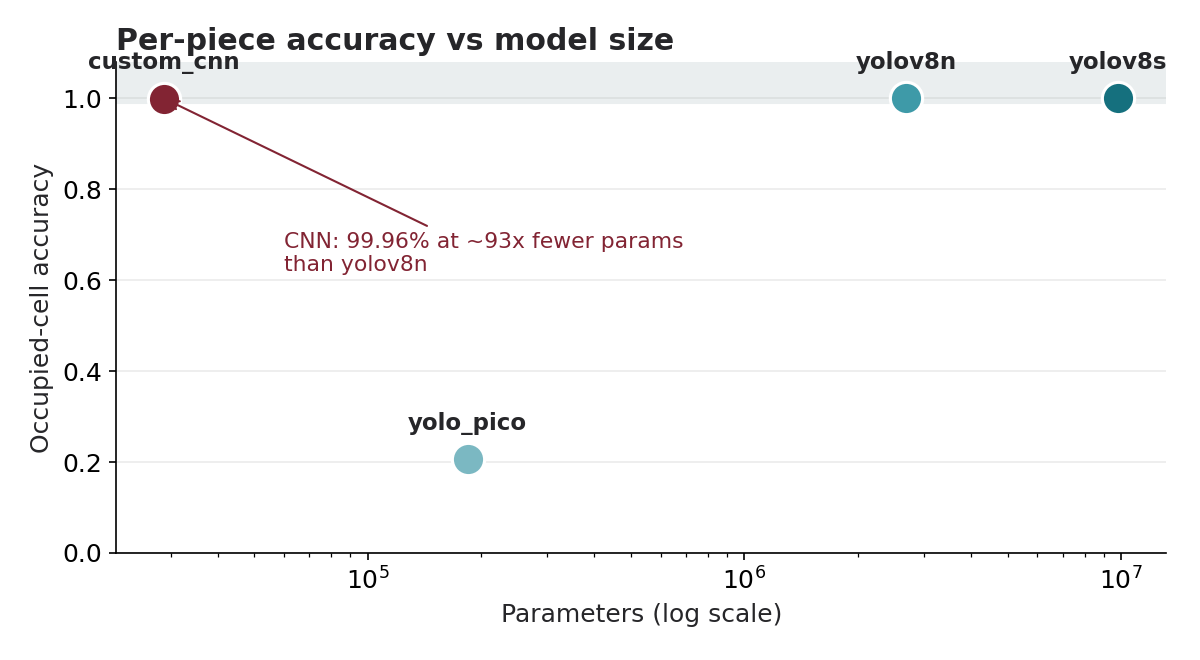
\includegraphics[width=\columnwidth]{acc_vs_params.png}
		\caption{Per-piece accuracy vs.\ model size (log scale). The custom CNN sits in the top-left: near-perfect accuracy at the smallest size.}
		\label{fig:acc}
	\end{figure}

	\begin{figure}[h]
		\centering
		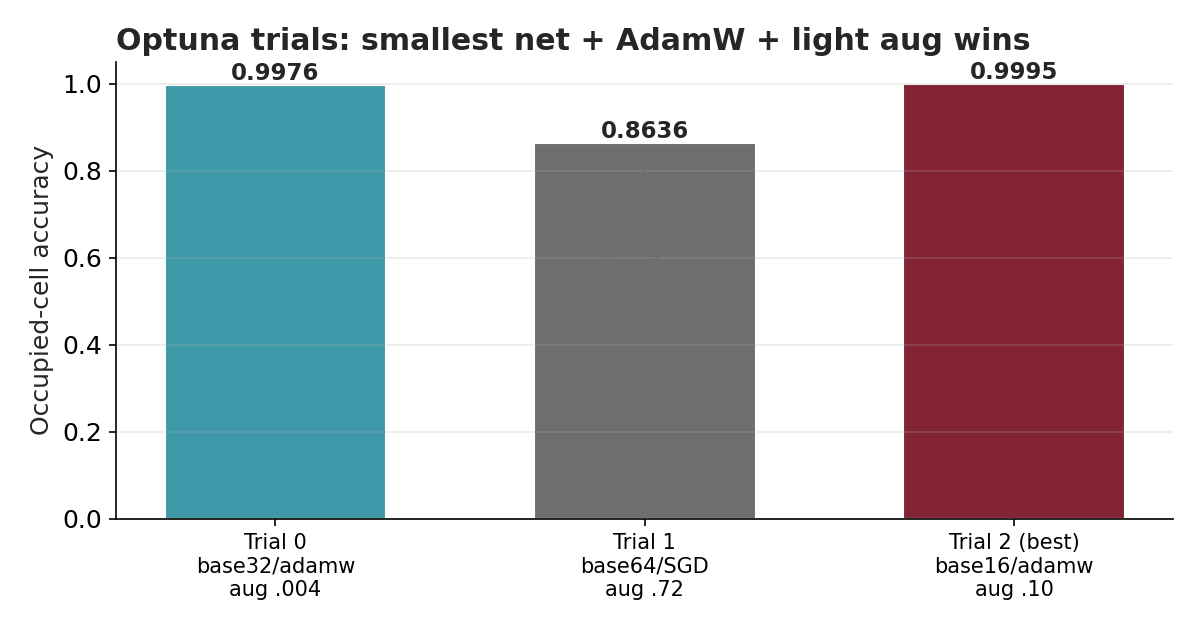
\includegraphics[width=\columnwidth]{hpo.png}
		\caption{CNN hyperparameter trials. AdamW with light augmentation on the smallest network wins; SGD with heavy augmentation collapses.}
		\label{fig:hpo}
	\end{figure}

	\subsection{Critical Discussion}

	\textbf{Which method is best, and why?} For this dataset the pretrained detectors are perfect, but the tiny CNN is only $0.04$ percentage points behind at roughly $1\%$ of the cost ($\sim 93\times$ fewer parameters than yolov8n, $\sim 8.5\times$ lower latency, $\sim 45\times$ smaller on disk). The reason the detectors win on raw accuracy is that the boxes are perfectly grid-aligned, so localization is trivial and only classification matters---something a COCO-pretrained backbone does flawlessly. But that same observation is why the detector is overkill here: when localization is free, the expensive part of detection is wasted.

	\textbf{Did the analysis produce a real insight?} Yes. The hyperparameter study (Fig.~\ref{fig:hpo}) shows three useful things: AdamW clearly beats SGD in this short-training regime; strong augmentation \emph{hurts} on clean rendered pieces (the heavy-augmentation trial dropped to $0.86$); and, surprisingly, the \emph{smallest} searched network was the best, which is why we ship a $28.8$k-parameter model. The pico experiment gives the clearest lesson: shrinking a detector to classifier size does not work---pico both collapses in accuracy and is \emph{slower} than nano, because reducing width does not remove the detection head's fixed overhead, and a sub-nano detector cannot learn from limited data in few epochs while a same-size classifier learns the task in a single epoch. In short, \emph{shrink the paradigm, not just the width}.

	\textbf{Where does it fail, and is it coherent with related work?} The CNN's efficiency depends on the $8\times8$ grid assumption, which is free here but not on a real photograph; this is exactly the regime where detectors are known to be necessary, so our conclusion is consistent with the literature rather than contradicting it. The hardest classes are the rarer ones (queens appear in under $1\%$ of cells), but on this clean data even those are essentially solved.

	\textbf{Limitations and future work.} The data is synthetic and grid-aligned, so the comparison should be read as ``when the board is already cropped''. A real-photo test set, full-data YOLO training with its own hyperparameter sweep, and a board$\to$FEN reconstruction step are natural extensions.

	\section{Conclusion}
	\label{sec:conclusion}

	We compared a tiny custom CNN classifier against YOLOv8 detectors for chess piece recognition on a shared synthetic dataset, using a fair occupied-cell metric and an explicit efficiency axis. The classifier matches the detectors' accuracy ($99.96\%$ vs.\ $100\%$) at a fraction of the size, latency, and disk footprint, while a from-scratch sub-nano detector fails outright. Our contribution is the controlled benchmark, the two-view data pipeline, and the hyperparameter analysis that explains the result. The practical takeaway is to match the model paradigm to the problem: for boards that can be cropped to a grid, a small classifier is the right choice, whereas a detector earns its cost only when the pieces must first be found in an unconstrained image.

	\section*{Acknowledgments}

	We thank the authors of the \textit{Chess Positions} dataset~\cite{koryakin2019chess} and the maintainers of PyTorch, Ultralytics, Optuna, and Kornia for their open-source tools.

	\bibliographystyle{ieeetr}
	\bibliography{references}

\end{document}
